\documentclass[]{article}
\usepackage{lmodern}
\usepackage{amssymb,amsmath}
\usepackage{ifxetex,ifluatex}
\usepackage{fixltx2e} % provides \textsubscript
\ifnum 0\ifxetex 1\fi\ifluatex 1\fi=0 % if pdftex
  \usepackage[T1]{fontenc}
  \usepackage[utf8]{inputenc}
\else % if luatex or xelatex
  \ifxetex
    \usepackage{mathspec}
  \else
    \usepackage{fontspec}
  \fi
  \defaultfontfeatures{Ligatures=TeX,Scale=MatchLowercase}
\fi
% use upquote if available, for straight quotes in verbatim environments
\IfFileExists{upquote.sty}{\usepackage{upquote}}{}
% use microtype if available
\IfFileExists{microtype.sty}{%
\usepackage{microtype}
\UseMicrotypeSet[protrusion]{basicmath} % disable protrusion for tt fonts
}{}
\usepackage[margin=1in]{geometry}
\usepackage{hyperref}
\hypersetup{unicode=true,
            pdftitle={App Sensory Analysis Bean to Bar Chocolate},
            pdfauthor={Johnnery Aldana},
            pdfborder={0 0 0},
            breaklinks=true}
\urlstyle{same}  % don't use monospace font for urls
\usepackage{graphicx,grffile}
\makeatletter
\def\maxwidth{\ifdim\Gin@nat@width>\linewidth\linewidth\else\Gin@nat@width\fi}
\def\maxheight{\ifdim\Gin@nat@height>\textheight\textheight\else\Gin@nat@height\fi}
\makeatother
% Scale images if necessary, so that they will not overflow the page
% margins by default, and it is still possible to overwrite the defaults
% using explicit options in \includegraphics[width, height, ...]{}
\setkeys{Gin}{width=\maxwidth,height=\maxheight,keepaspectratio}
\IfFileExists{parskip.sty}{%
\usepackage{parskip}
}{% else
\setlength{\parindent}{0pt}
\setlength{\parskip}{6pt plus 2pt minus 1pt}
}
\setlength{\emergencystretch}{3em}  % prevent overfull lines
\providecommand{\tightlist}{%
  \setlength{\itemsep}{0pt}\setlength{\parskip}{0pt}}
\setcounter{secnumdepth}{0}
% Redefines (sub)paragraphs to behave more like sections
\ifx\paragraph\undefined\else
\let\oldparagraph\paragraph
\renewcommand{\paragraph}[1]{\oldparagraph{#1}\mbox{}}
\fi
\ifx\subparagraph\undefined\else
\let\oldsubparagraph\subparagraph
\renewcommand{\subparagraph}[1]{\oldsubparagraph{#1}\mbox{}}
\fi

%%% Use protect on footnotes to avoid problems with footnotes in titles
\let\rmarkdownfootnote\footnote%
\def\footnote{\protect\rmarkdownfootnote}

%%% Change title format to be more compact
\usepackage{titling}

% Create subtitle command for use in maketitle
\providecommand{\subtitle}[1]{
  \posttitle{
    \begin{center}\large#1\end{center}
    }
}

\setlength{\droptitle}{-2em}

  \title{App Sensory Analysis Bean to Bar Chocolate}
    \pretitle{\vspace{\droptitle}\centering\huge}
  \posttitle{\par}
    \author{Johnnery Aldana}
    \preauthor{\centering\large\emph}
  \postauthor{\par}
      \predate{\centering\large\emph}
  \postdate{\par}
    \date{21/4/2020}


\begin{document}
\maketitle

\hypertarget{objective}{%
\subsection{Objective}\label{objective}}

This Aplication have like objetive help in the test sensory analysis
``Bean to Bar'' chocolates.

``Bean to Bar'' chocolates are chocolates made with fine aroma cacao.
This cacao represents just 5\% of world production and is produced in
very few places.

``Bean to Bar'' chocolates are similar to high-end wines and have unique
flavors depending on the origin of the beans. Venezuela is the country
with the largest variety of cocoa with fine aroma. The famous porcelain
cocoa, chuao, ocumare, patanemo, caruao among many others, located on
the map below.

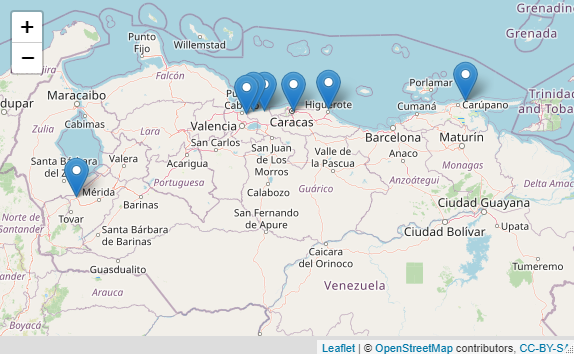
\includegraphics[width=5.74in]{CACAO_VENEZUELA}

\hypertarget{sensory-analysis}{%
\subsection{Sensory Analysis}\label{sensory-analysis}}

Sensory analysis is the use of the 5 senses (smell, sight, hearing,
touch and taste) to evaluate, detect and scrutinize the different
features that characterize chocolate.

In the sensory evaluation of the attributes of flavor and aroma, the
descriptors of the chocolate are taken into account, which are: Sweet,
Salty, Bitter, Astringent, Dried\_Fruits, Citrus, Species, etc.

When tasting a chocolate our senses are activated and together with our
memories of flavors and aroma we can determine the descriptores of
chocolate. Then we can assign a value to each descriptor and build a
sensory profile diagram. As we show below.

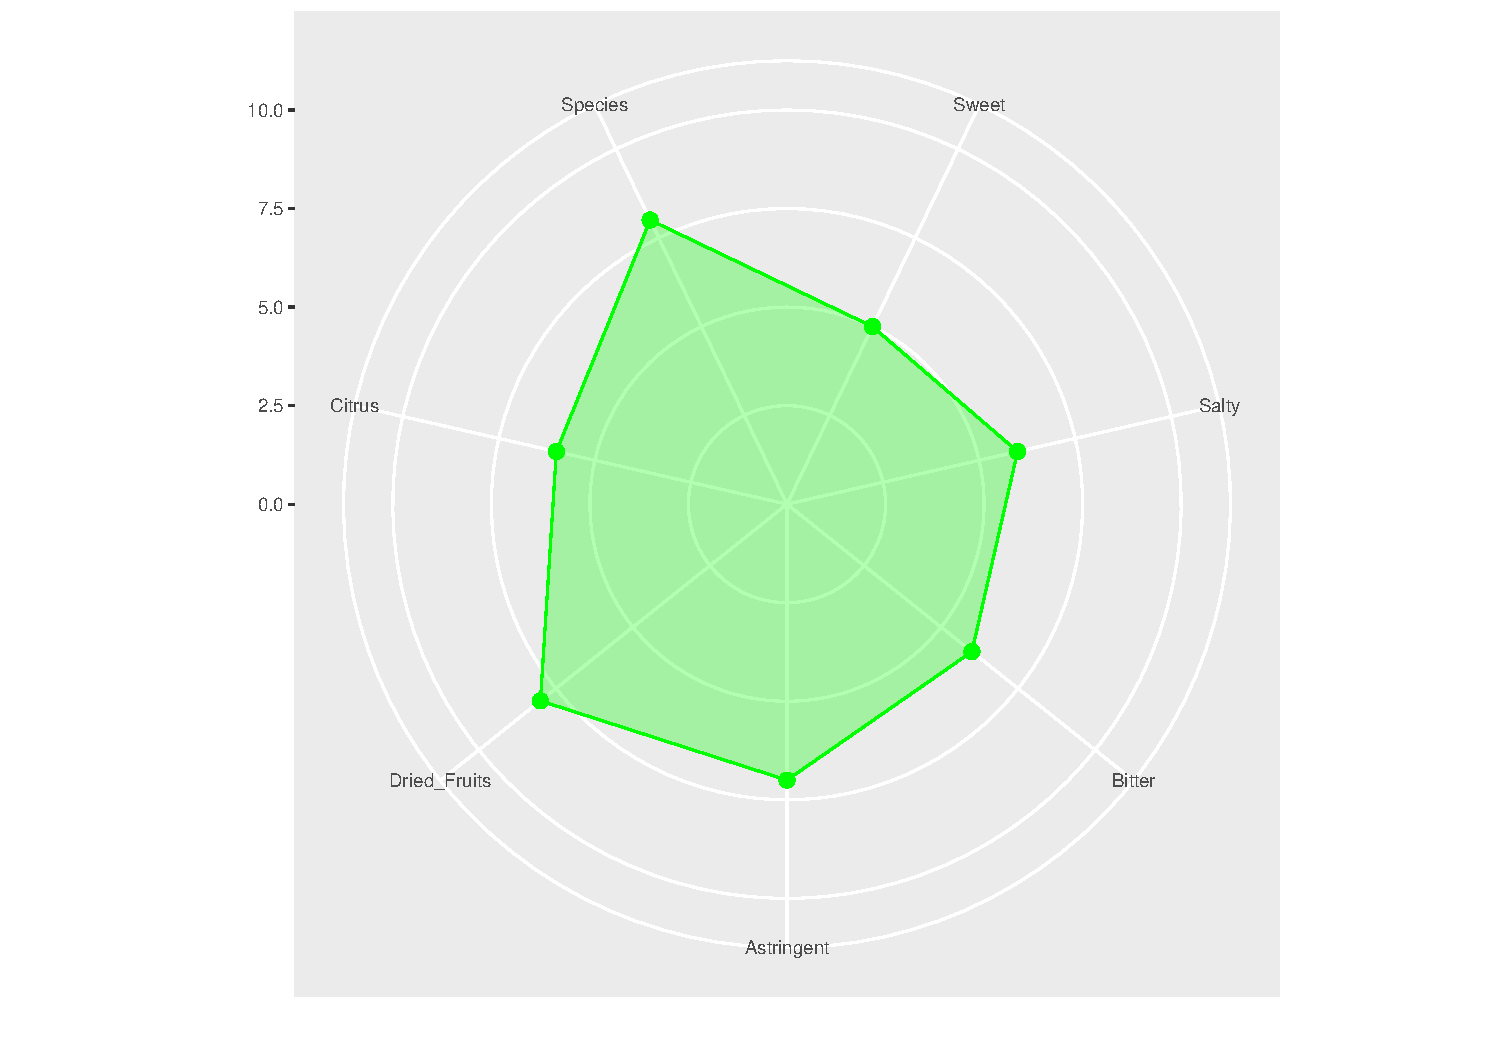
\includegraphics{App_Test_Sensory_files/figure-latex/unnamed-chunk-2-1.pdf}

\hypertarget{app-sensory-analysis-bean-to-bar-chocolate}{%
\subsection{App Sensory Analysis Bean to Bar
Chocolate}\label{app-sensory-analysis-bean-to-bar-chocolate}}

Our application helps interactively and in a very simple way with the
sensory analysis process allowing the taster to fill in the values on
the left side and generating the sensory profile diagram on the right
side. As can be seen in the following figure.

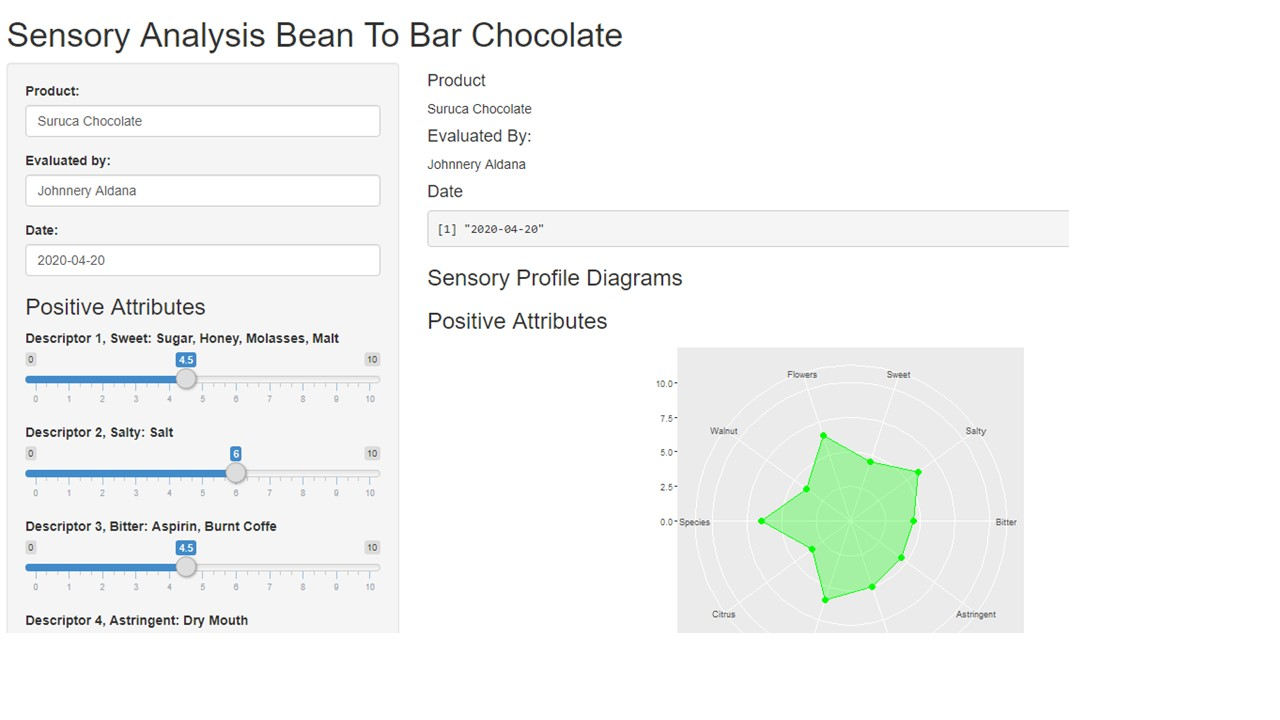
\includegraphics[width=12.8in]{APP_Test_Sensory}

\hypertarget{app-sensory-analysis-bean-to-bar-chocolate-1}{%
\subsection{App Sensory Analysis Bean to Bar
Chocolate}\label{app-sensory-analysis-bean-to-bar-chocolate-1}}

We can also evaluate the flaws in the flavor that the chocolate may
present, such as: Metal, Moisture, powder, over-fermented, etc.

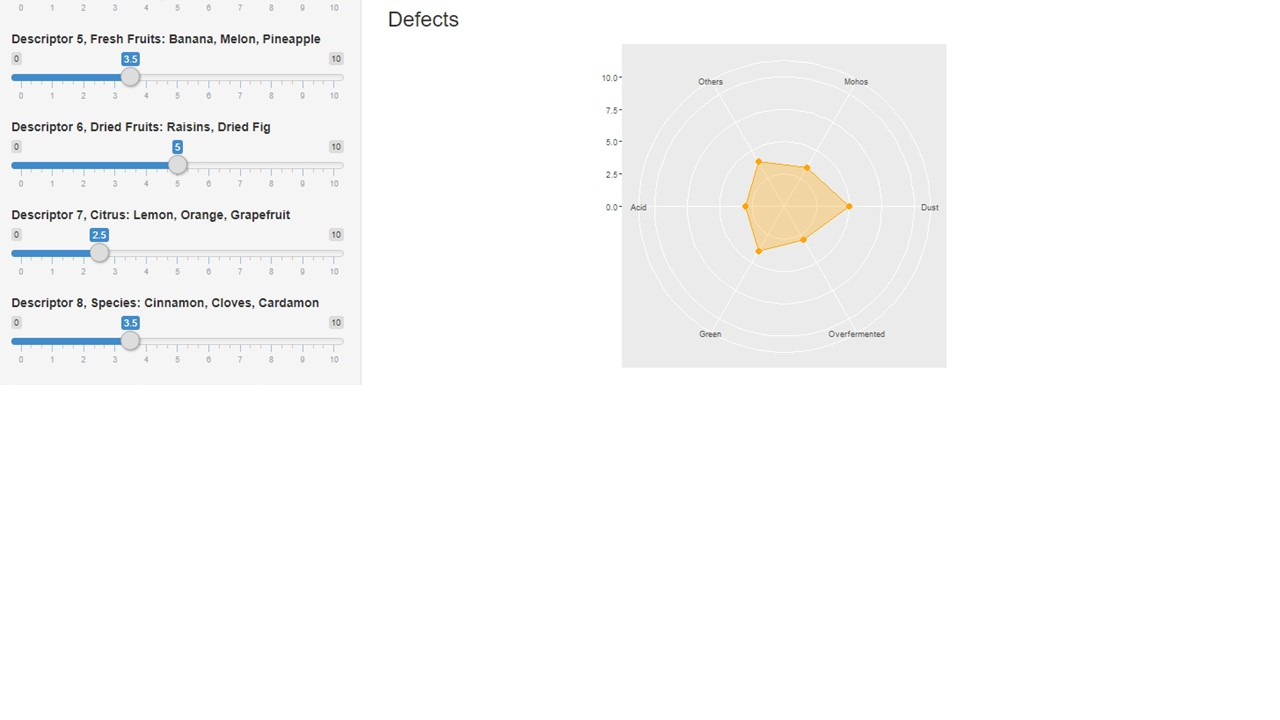
\includegraphics[width=12.8in]{App_Test_Sensory_2}

Thanks so much


\end{document}
